\documentclass[portuges,]{article}
\usepackage[T1]{fontenc}
\usepackage{lmodern}
\usepackage{amssymb,amsmath}
\usepackage{booktabs}
\usepackage{ifxetex,ifluatex}
\usepackage{fixltx2e} % provides \textsubscript
% Set line spacing
% use upquote if available, for straight quotes in verbatim environments
\IfFileExists{upquote.sty}{\usepackage{upquote}}{}
\ifnum 0\ifxetex 1\fi\ifluatex 1\fi=0 % if pdftex
  \usepackage[utf8]{inputenc}
\else % if luatex or xelatex
  \ifxetex
    \usepackage{mathspec}
    \usepackage{xltxtra,xunicode}
  \else
    \usepackage{fontspec}
  \fi
  \defaultfontfeatures{Mapping=tex-text,Scale=MatchLowercase}
  \newcommand{\euro}{€}
\fi
% use microtype if available
\IfFileExists{microtype.sty}{\usepackage{microtype}}{}
\usepackage[margin=1in]{geometry}
\usepackage{graphicx}
% Redefine \includegraphics so that, unless explicit options are
% given, the image width will not exceed the width of the page.
% Images get their normal width if they fit onto the page, but
% are scaled down if they would overflow the margins.
\makeatletter
\def\ScaleIfNeeded{%
  \ifdim\Gin@nat@width>\linewidth
    \linewidth
  \else
    \Gin@nat@width
  \fi
}
\makeatother
\let\Oldincludegraphics\includegraphics
{%
 \catcode`\@=11\relax%
 \gdef\includegraphics{\@ifnextchar[{\Oldincludegraphics}{\Oldincludegraphics[width=\ScaleIfNeeded]}}%
}%
\ifxetex
  \usepackage[setpagesize=false, % page size defined by xetex
              unicode=false, % unicode breaks when used with xetex
              xetex]{hyperref}
\else
  \usepackage[unicode=true]{hyperref}
\fi
\hypersetup{breaklinks=true,
            bookmarks=true,
            pdfauthor={},
            pdftitle={Bio 208 - Lista 5},
            colorlinks=true,
            citecolor=blue,
            urlcolor=blue,
            linkcolor=magenta,
            pdfborder={0 0 0}}
\urlstyle{same}  % don't use monospace font for urls
\setlength{\parindent}{0pt}
\setlength{\parskip}{6pt plus 2pt minus 1pt}
\setlength{\emergencystretch}{3em}  % prevent overfull lines
\setcounter{secnumdepth}{0}
\ifxetex
  \usepackage{polyglossia}
  \setmainlanguage{}
\else
  \usepackage[portuges]{babel}
\fi

%%% Change title format to be more compact
\usepackage{titling}
\setlength{\droptitle}{-2em}
  \title{Bio 208 - Lista 5}
  \pretitle{\vspace{\droptitle}\centering\huge}
  \posttitle{\par}
  \author{}
  \preauthor{}\postauthor{}
  \predate{\centering\large\emph}
  \postdate{\par}
  \date{Novembro 2014}




\begin{document}

\maketitle


Uma pesquisadora está interessada em estudar efeitos de mudanças
climáticas na morfologia craniana de esquilos do gênero Tamias (esquilos
parecidos com o Tico e Teco). Para isso ela mediu 4 caracteres cranianos
de forma não invasiva (via tomografia computadorizada) em 500 indivíduos
desta espécie. Os caracteres medidos estão esquematicamente apresentados
em um crânio de esquilo na figura abaixo. Do lado esquerdo podemos ver
as correlações entre os diferentes caracteres medidos. Sendo os valores
acima da diagonal os valores de correlação e os histogramas apresentados
na diagonal representam a distribuição das medidas tomadas para cada
medida. Os gráficos abaixo da diagonal representam os valores observados
entre duas medidas, isto é, cada ponto é um indivíduo medido. No eixo x
temos o valor dele na medida indicada em x e no eixo y o valor observado
neste indivíduo para a medida indicada no eixo y.

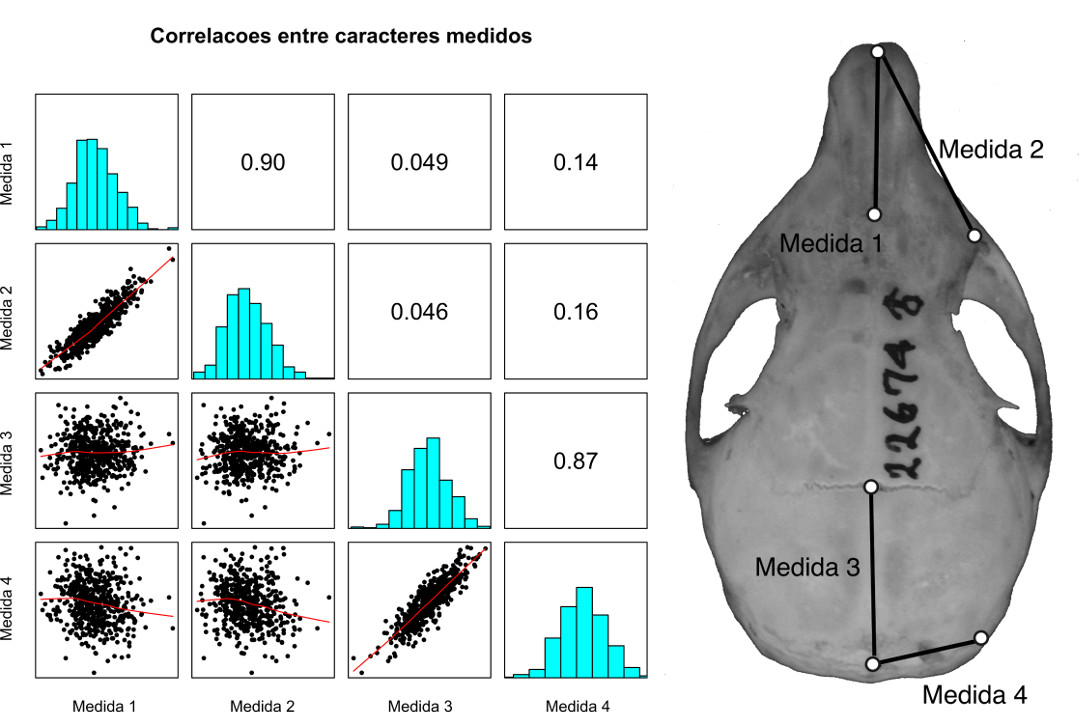
\includegraphics{/home/diogro/projects/Bio208/static/pdfs/roteiros_listas/fig1.jpg}

Com estes dados ela calculou uma matriz de variância/covariância
genética aditiva e as médias de cada medida (Tabelas 1 e 2)

\begin{table}[ht]
\centering
\begin{tabular}{rrrrr}
  \toprule
 & Medida\_1 & Medida\_2 & Medida\_3 & Medida\_4 \\ 
  \midrule
Medida\_1 & 1.02 & 0.84 & 0.04 & -0.10 \\ 
  Medida\_2 & 0.84 & 0.86 & 0.03 & -0.10 \\ 
  Medida\_3 & 0.04 & 0.03 & 0.61 & 0.48 \\ 
  Medida\_4 & -0.10 & -0.10 & 0.48 & 0.51 \\ 
   \bottomrule
\end{tabular}
\caption{Matriz G estimada para a população} 
\end{table}\begin{table}[ht]
\centering
\begin{tabular}{rrrrr}
  \toprule
 & Medida\_1 & Medida\_2 & Medida\_3 & Medida\_4 \\ 
  \midrule
Média & 8.93 & 10.69 & 9.58 & 5.81 \\ 
   \bottomrule
\end{tabular}
\caption{Média para as quatro medidas antes da seleção} 
\end{table}

\newpage

A partir destes dados, tal pesquisadora (e você também) pode então
analisar quais efeitos que diferentes regimes seletivos teriam para a
morfologia craniana desta espécie. Por exemplo, qual efeito esperaríamos
para as médias caso essa população sofra seleção direcional pelo
seguinte gradiente de seleção, que atua somente sobre a medida 1:

\begin{table}[ht]
\centering
\begin{tabular}{rrrrr}
  \toprule
 & Medida\_1 & Medida\_2 & Medida\_3 & Medida\_4 \\ 
  \midrule
Gradiente de Seleção & 1.00 & 0.00 & 0.00 & 0.00 \\ 
   \bottomrule
\end{tabular}
\caption{Gradiente de seleção hipotético atuando sobre a medida 1} 
\end{table}

Q1. Qual é a resposta esperada a esta seleção direcional? (calcule o
$\Delta Z$ e as novas médias esperadas após a seleção)

Agora faça o mesmo exercício baseado nos cinco gradientes de seleção
abaixo:

\begin{table}[ht]
\centering
\begin{tabular}{rrrrrr}
  \toprule
 & Beta\_1 & Beta\_2 & Beta\_3 & Beta\_4 & Beta\_5 \\ 
  \midrule
Medida\_1 & 0.00 & 0.00 & 0.00 & 1.00 & 1.00 \\ 
  Medida\_2 & 1.00 & 0.00 & 0.00 & 1.00 & -1.00 \\ 
  Medida\_3 & 0.00 & 1.00 & 0.00 & -1.00 & 1.00 \\ 
  Medida\_4 & 0.00 & 0.00 & 1.00 & -1.00 & -1.00 \\ 
   \bottomrule
\end{tabular}
\end{table}

Q2. Quais seriam as respostas esperadas para estes gradientes de
seleção? (novamente calcule o $\Delta Z$ e as novas médias da população
para cada vetor de seleção)

Q3. Baseado nestas observações discuta:

\begin{enumerate}
\def\labelenumi{\alph{enumi})}
\item
  Você acha que a seleção natural é um agente otimizador ultra-eficiente
  capaz de otimizar cada parte de um organismo? (sim, não, porque?)
\item
  O que você entende por restrição evolutiva e quais as suas
  consequências para a evolução?
\item
  Comparando-se os gradientes de seleção 5 e 6 e as respostas produzidas,
  em qual dos dois casos a restrição evolutiva foi maior? Por que?
\item
  Qual a relação disto com a teoria de modularidade?
\end{enumerate}

\end{document}
